% Appendix A

\chapter{Analytic Expression for the Ly$\alpha$ Spectrum emerging from Rotating Cloud}\label{sec:app} % For referencing this appendix elsewhere, use \ref{AppendixA}

\lhead{Appendix \emph{Analytic Expression for the Ly$\alpha$ Spectrum emerging from Rotating Cloud}} % This is for the header on each page - perhaps a shortened title

Ly$\alpha$ scattering through an optically thick gas cloud that is
undergoing solid-body rotation (i.e. in which the angular speed around the
rotation axis is identical for each hydrogen atom) proceeds identical
as in a static cloud. In order to compute the spectrum emerging from a rotating cloud, we sum
the spectra emerging from all surface elements of the cloud, weighted by their intensity.
We adopt the geometry shown in Fig~\ref{fig:scheme} to derive an analytic expression of this emerging spectrum,
Note that this geometry differs from the scheme shown in Fig~1 in the main body of
the thesis.
%
\begin{figure*}[h]
\centerline{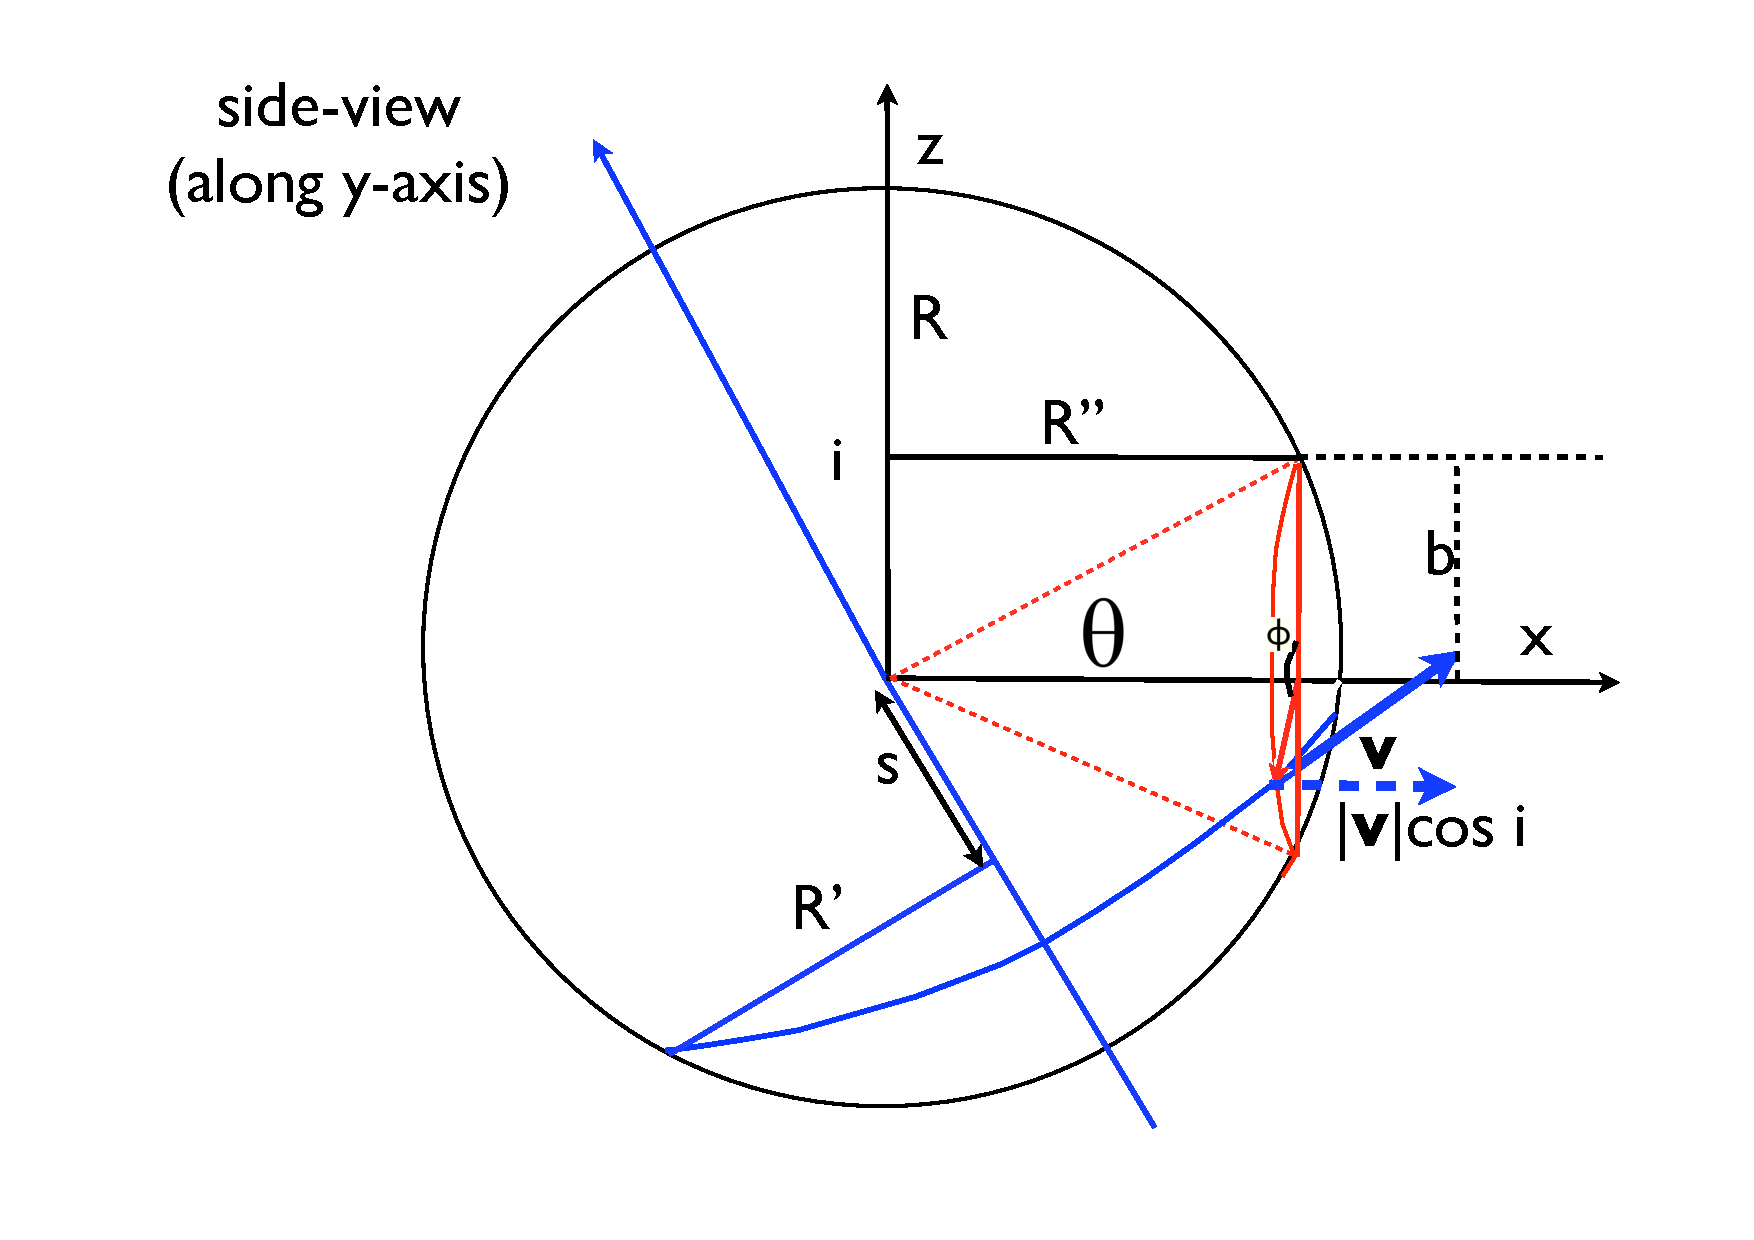
\includegraphics[width=80mm]{../Figures/fig11a.pdf}
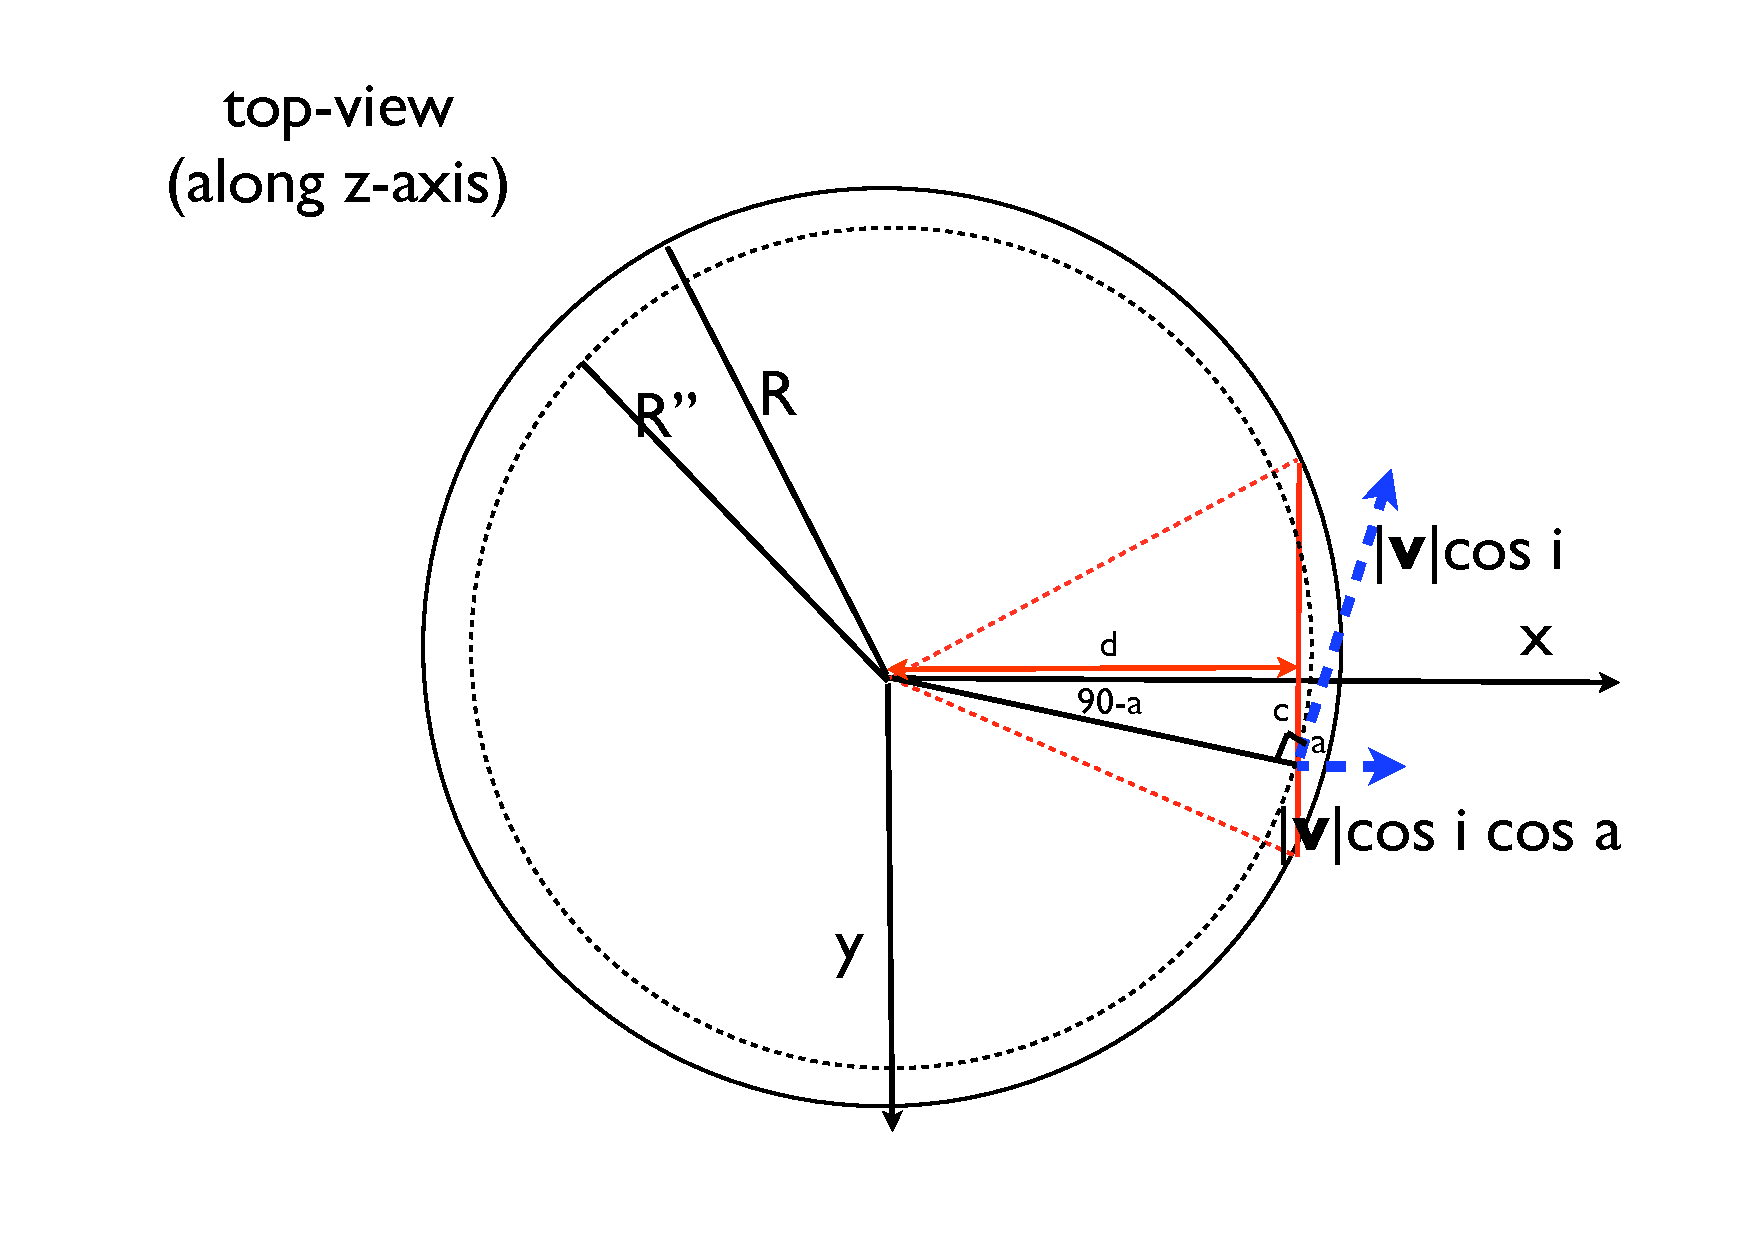
\includegraphics[width=80mm]{../Figures/fig11b.pdf}}
\caption[]{Adopted geometry for evaluating the analytic spectrum.}
\label{fig:scheme}
\end{figure*}
%
The sightline to the observer \& rotation axis define the $x-z$ plane.
The {\it left panel} in Fig~\ref{fig:scheme} shows the view from the $y$-axis.
The observer sits along the $x$ axis.
The rotation axis makes an angle $i$ with respect to the $z$-axis.
We sum up spectra from individual patches by integrating over the
impact parameter $b$, and angle $\phi$.
Each $(b,\phi)$ corresponds to a point on the sphere.
This point has a velocity vector ${\bf v}(b,\phi,i)$, which we denote
with ${\bf v}$ for brevity. The magnitude of ${\bf v}$ is $|{\bf v}|=V_{\rm max}R'/R$. Here $R'=\sqrt{R^2 -s^2}$, in which $s$ denotes the distance of the point $(b,\phi)$ to the plane perpendicular to the rotation axis and through the origin (see the {\it left panel} of Fig~\ref{fig:scheme}). This distance $s$ is given by $s=|-\sin i\sqrt{R^2-b^2}+ b \cos \phi \cos i|$.\\
The spectrum of the flux emerging from the surface at point $(b,\phi)$ is
\begin{displaymath}
J(x,b,\phi,i)=\frac{\sqrt{\pi}}{\sqrt{24}a\tau_0}\Bigg{(}\frac{(x-x_{\rm
b})^2}{1+{\rm cosh}\Big{[}\sqrt{\frac{2\pi^3}{27}}\frac{|(x
-x_{\rm b})^3|}{a\tau_0}\Big{]}}\Bigg{)},
\end{displaymath}
%
where $x_b\equiv v_{b}/v_{\rm th}$, and $v_b$ is the component of ${\bf v}$ projected onto the line-of-sight. This component is given by
\begin{equation}
v_{\rm b}(b,\phi,i)=V_{\rm max}\frac{\sqrt{R^2 -s^2}}{R}\cos i \hs
\cos a,
\end{equation}
where $\beta = 90^{\circ}-a$. The factor $\cos i$ accounts for the projection onto the $x-y$ plane, and the factor $\cos a$ for the subsequent projection onto the line-of-sight. The {\it right panel} of Fig.~\ref{fig:scheme} shows that this angle $a$ can be computed from
%
\begin{equation}
\tan \beta =\tan[90^{\circ}-a]=\frac{c}{d}=\frac{ b\sin \phi}{\sqrt{R^2 -b^2}},
\end{equation}
%
In order to compute to total intensity we integrate over $b$ and
$\phi$ with a weight given by the surface brightness of the
sphere at $(b,\phi)$, $S(b,\phi)$.
\begin{displaymath}
J(x,i)=2\pi \int_0^Rdb \hs b \int_0^{2\pi}d\phi \hs
S(b,\phi)J(x,b,\phi,i) \approx 2\pi \int_0^Rdb \hs b
\int_0^{2\pi}d\phi \hs J(x,b,\phi,i)\\ \nonumber.
\end{displaymath}
%
In the last expression we assume that $S(b,\phi)$ is constant.
This corresponds to $I(\mu) \propto \mu$ at the surface, where $\mu$
denotes the cosine of the angle of the propagation direction of the
outgoing photon and the normal to the spheres surface: a fixed $db$
corresponds to a physical length $ds = db/\mu$ on the sphere.
If $I(\mu)$ were constant, this would imply that the sphere should
appear brighter per unit $b$.
A constant surface brightness profile requires the directional
dependence for $I(\mu) \propto \mu$ to correct for this.
Indeed, this is what is expected for the escape of Ly$\alpha$ photons
from static, extremely opaque media (see \citet{Ahn01}; their
Fig~4 and accompanying discussion).
It is worth stressing that this derivation should not be viewed as a
complete analytic calculation, and we do not expect perfect agreement:
we {\it assumed} a functional form for the surface brightness profile
[or for $I(\mu)$]. Moreover, $I(\mu)$ itself may depend on frequency $x$. In other words, analytic solutions exist for $J(x) =
\int_0^1 I(x,\mu) d\mu$ at the boundary of the sphere, and {\it approximate}
expressions for $I(\mu) =\int dx I(x,\mu)$, but {\it not} for $I(x,\mu)$
itself. The spectra we obtained from the Monte-Carlo calculations naturally include the proper $I(x,\mu)$, and are therefore expected to be more accurate.
To further test the assumption of scattering in a rotating medium proceeding
as in a static medium we compute the distribution of the outgoing
angles $\mu$. The results are shown in Figure \ref{fig:surface}; it
shows that the distribution for $\mu$ is independent of the rotational
velocity and the location over the sphere. The only dependence comes
with $\tau_{H}$. For higher values of the optical depth the
distribution gets closer to $I(\mu)\propto \mu$ as expected for a
static medium \citep{Ahn01}.
%
\begin{figure*}[h]
\centerline{
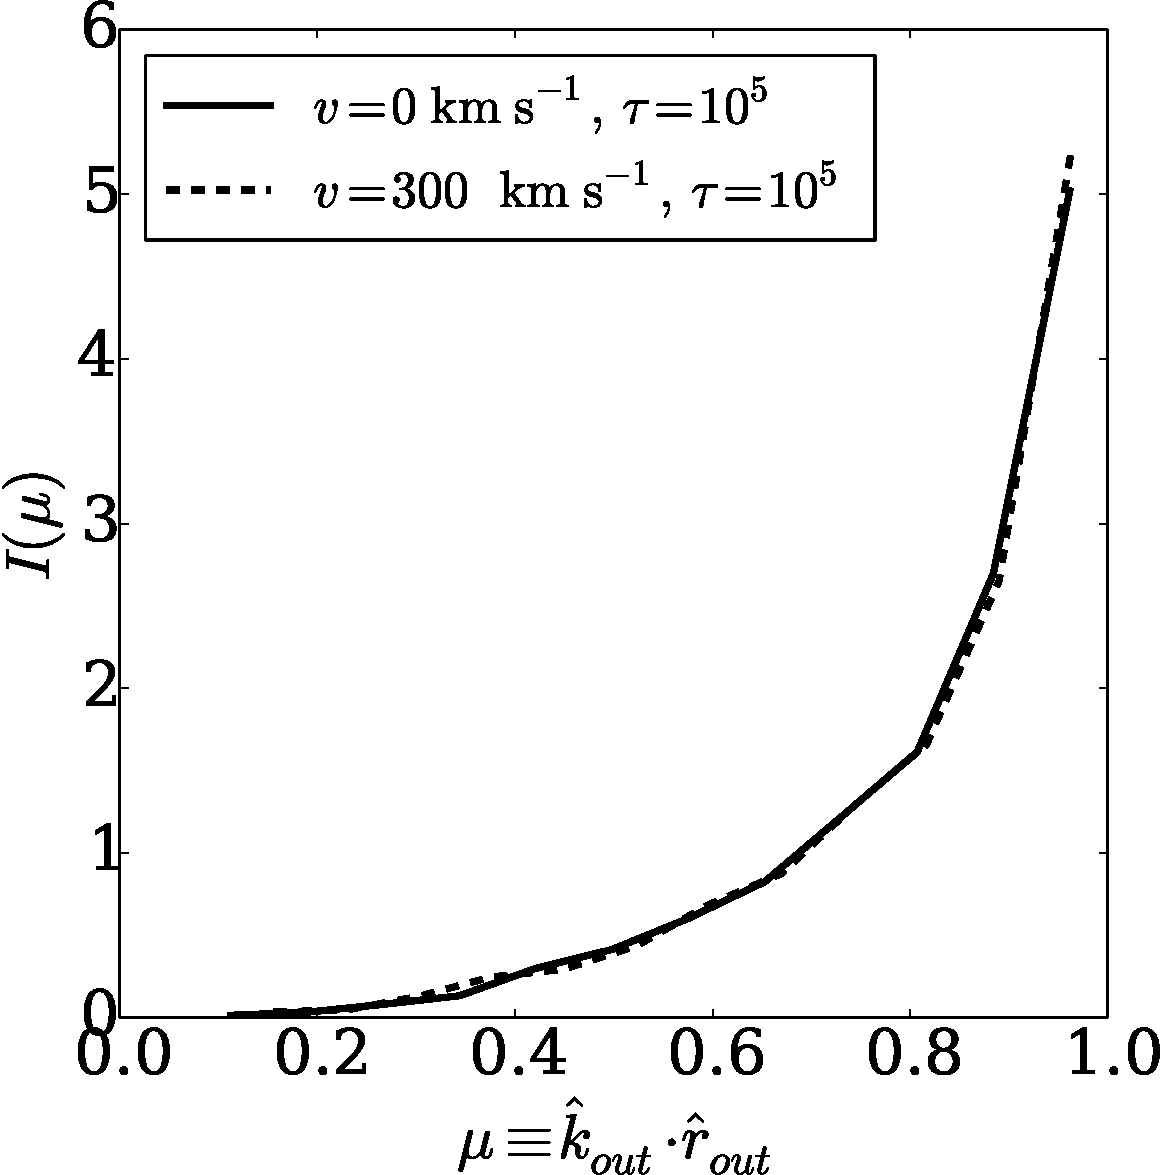
\includegraphics[width=0.30\textwidth]{../Figures/fig12a.pdf}
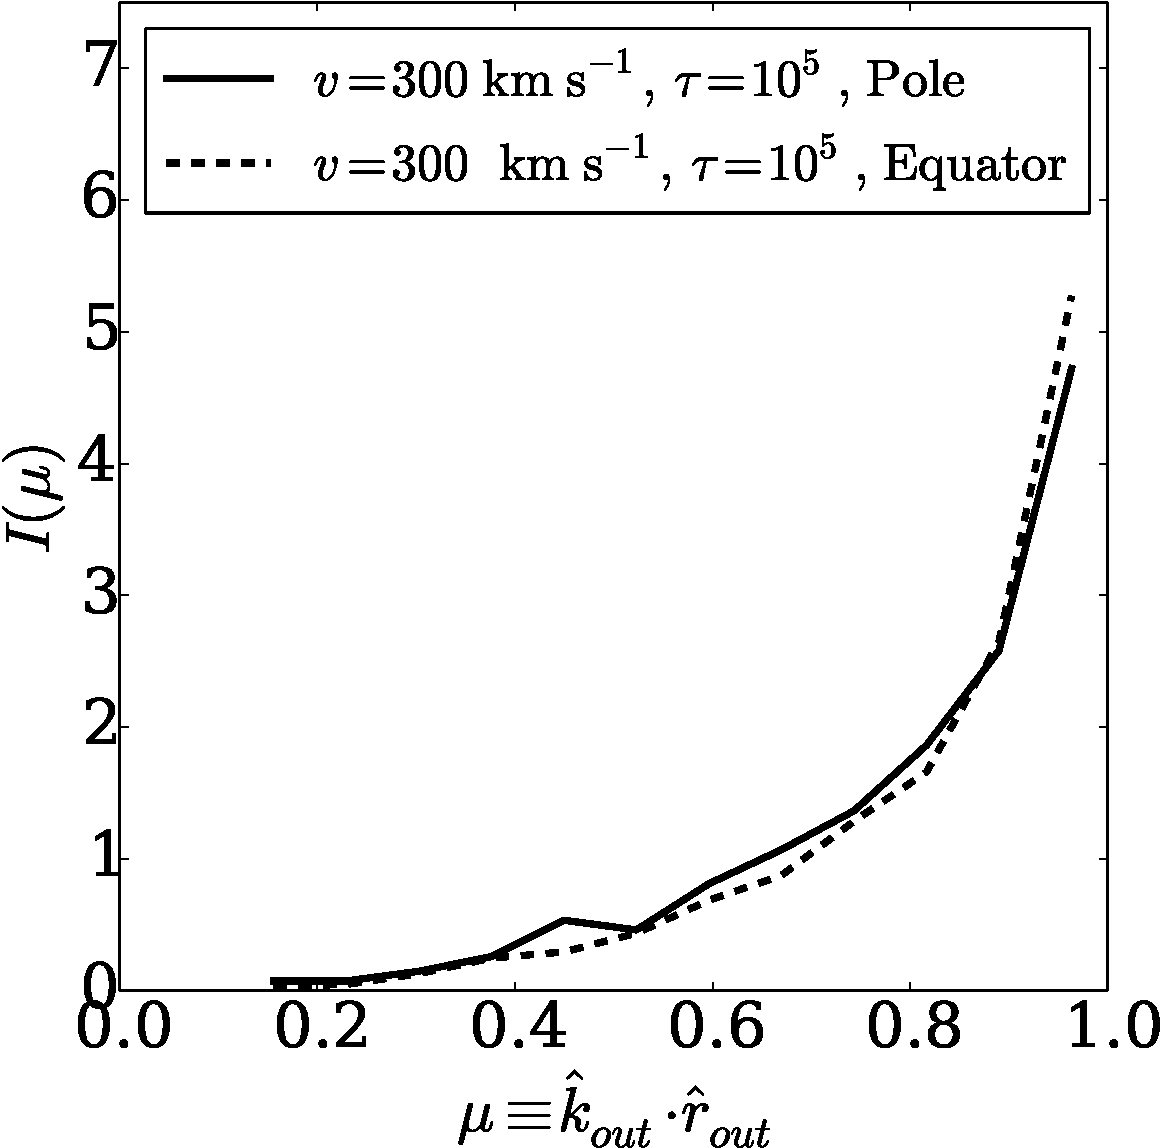
\includegraphics[width=0.30\textwidth]{../Figures/fig12b.pdf}
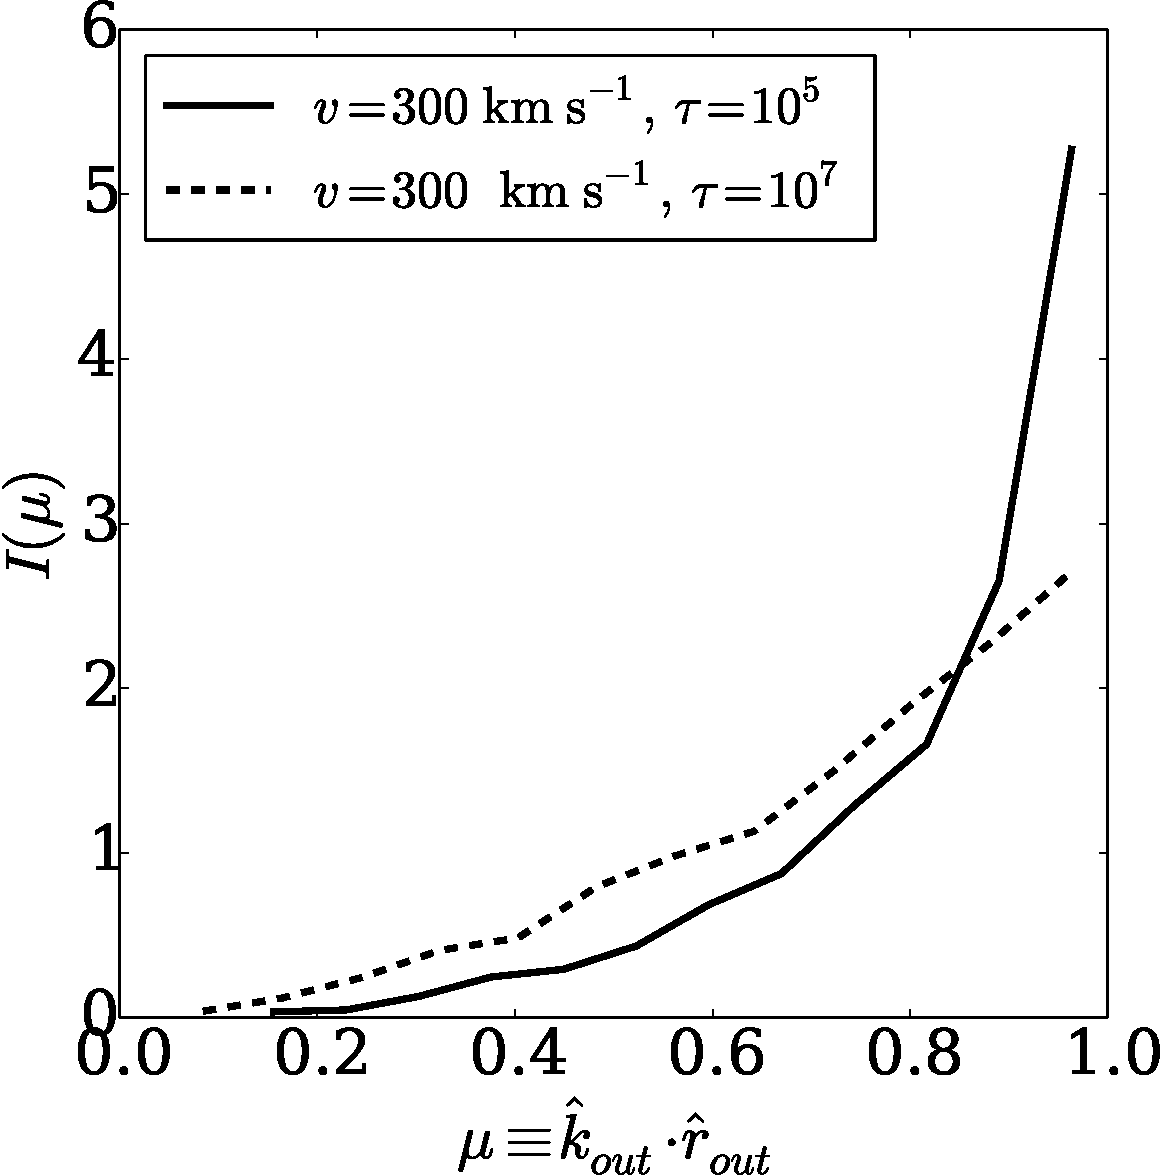
\includegraphics[width=0.30\textwidth]{../Figures/fig12c.pdf}}
\caption[]{Distribution of the cosine of the angle between the
propagation direction and a vector normal to the sphere's
surface. The distributions have been normalized to unity. Left
panel: different rotational velocities; middle panel: different
viewing angles; right panel: different optical depths. Only the
optical depth has an effect on the distribution of outogoing
directions. This is consistent with the assumption that \lya
scattering in a medium with solid body rotation proceeds as in a
static medium.}
\label{fig:surface}
\end{figure*}
%
